\documentclass[a4paper,11pt]{article} %, landscape report

\usepackage[T1]{fontenc}
\usepackage[utf8x]{inputenc}

%Selon les goûts: times palatino bookman newcent chancery helvet avant fourier kpfonts cmbright
%\usepackage{avant}

%\usepackage[hmargin=2cm,vmargin=2cm]{geometry}
%\usepackage{multicol}
%\setlength{\columnsep}{1cm}

\usepackage{graphicx}
\usepackage{xcolor}
\usepackage{multicol}\setlength{\columnsep}{1cm}

\usepackage{amsmath,amssymb,amsfonts,makeidx}
\usepackage{stmaryrd}% crochets «intervalles d'entiers»
%\newcommand{\B}{\mathbb{B}}
\usepackage{tikz}


\newcommand{\vesp}{\vspace*{0.2em}}
\newcommand{\VESP}{\vspace*{0.8em}}

\usepackage{hyperref}
\hypersetup{colorlinks=true, 
            linkcolor=violet,
            urlcolor=teal,
            citecolor=olive,
            }
\newcommand{\www}[2]{\href{#1}{\nolinkurl{#2}}}
%black, blue, brown, cyan, darkgray, gray, green, lightgray, lime, magenta, olive, orange, pink, purple, red, teal, violet, white, yellow
%\urlstyle{same}% Pas stylés \og URL

%\usepackage[nosort]{cite}

%\newcommand{\1}{\textcircled{\small 1}}
%\newcommand{\2}{\textcircled{\small 2}}

\usepackage[french]{babel} \frenchbsetup{StandardLists=true}
\usepackage[autolanguage]{numprint}
\DecimalMathComma

\AddThinSpaceBeforeFootnotes
\FrenchFootnotes

% =================================================================================================
\title{État de l'art du Projet d'initiation à la Recherche\\M2 I2A}
\author{Jean-Marc Gervais\\[0.6em]
Encadré par M. Jean-François Couchot\\
\small Institut FEMTO-ST, UMR 6174 CNRS -- DISC Équipe AND}
\date{$15$ janvier $2\,020$}

\begin{document}%\setlength\parindent{5mm}
\maketitle
%%
\section*{\center Étendre la méthode RAPPOR aux données longitudinales de localisation\\[1cm]
-- Étude bibliographique préliminaire --}
%%
\thispagestyle{empty}
\newpage
%%
\tableofcontents
\newpage
\section{Introduction}
Les terminaux mobiles comme les smartphones sont utilisés massivement comme supports d'\textbf{applications qui offrent un service personnalisé} en s'appuyant sur l'\textbf{analyse du comportement individuel} de l'utilisateur. 
Cela renforce la nécessité de \textbf{protéger les données personnelles}, spécialement celles \textbf{de localisation}. 
Ces dernières sont particulièrement sensibles, sans que l'on n'en soit conscient la plupart du temps.

Mais leur richesse peut également être utilisée à bon escient, pour analyser, optimiser ou inférer, notamment au bénéfice direct de l'utilisateur. 
Alors, que ce soit d'un point de vue éthique ou par intérêt commercial ---~pour ne pas perdre la précieuse confiance des clients~--- la confidentialité doit être respectée. 
En fait, on verra qu'il est nécessairement affaire de compromis entre le respect de la sphère privée et la conservation ou la diffusion d'informations suffisamment exploitables.

Pour quantifier la garantie offerte ou au contraire la perte de confidentialité, des définitions précises seront nécessaires.
Le défi sera de les garder compréhensible par l'utilisateur non spécialiste, qui devrait pouvoir arbitrer.

Enfin, cette analyse devra également déboucher sur des applications pratiques et des outils qui facilitent leur mise en œuvre. 
Nous nous intéresserons particulièrement à la méthode RAPPOR (\textit{Randomized Aggregatable Privacy-Preserving Ordinal Response}), afin d'être en mesure d'envisager ultérieurement son adaptation aux données longitudinales\footnote{On désigne ainsi les relevés \og au fil du temps\fg{} sur une durée relativement longue, en opposition aux données dites transversales, recueillies sur une période courte.} de localisation.
%% ========================================================================================== %%
%%
%\section{Problématique}
%%
%
\subsection{Contexte}
%
Même si la notion de confidentialité recouvre un cadre plus large, nous nous intéressons principalement à la protection des données exploitées par les applications offrant un service à l'utilisateur basé sur la localisation (\textbf{données géographiques}, mais également \textbf{temporelles}).
Nous désignerons leurs fournisseurs par l'abréviation anglophone \textbf{LBS} (pour \emph{\textbf{Location-Based Services}}). 
Il peut s'agir notamment d'outils de navigation en temps réel, de prévision météo, proposant des lieux intéressants, ou indiquant la proximité d'autres utilisateurs à rencontrer. 
On pense également à toute collecte massive d'informations, qu'il s'agisse de consommations énergétiques, de conditions de circulation, de comportements (\emph{smart cities}, \emph{smart grid}, analyse de \og connaissance client\fg{}\footnote{L'exempe de Flux Vision d'Orange nous concerne tout particulièrement :\newline \url{https://www.orange-business.com/fr/produits/flux-vision}}, de données de santé (prévention, suivis épidémiologiques), etc.

Nous ne traitons pas ici des attaques utilisant des failles logicielles, l'ingénierie sociale ou des programmes malveillants, qui ont leurs réponses spécifiques, indépendantes de notre problématique. L'adversaire envisagé est un individu quelconque ayant accès aux données, simplement \og un peu trop curieux\fg{}, autrement dit quelqu'un qui cherche à obtenir des informations qui n'avaient pas vocation à être accessibles au départ. Il est supposé disposer d'accès à des bases de données externes et ses \og attaques\fg{} seront des exploitations calculatoires des réponses qu'on accepte de lui fournir.
%
\subsection{Critères d'analyse}
%
On distingue la \textbf{phase de collecte} (envoi du terminal de l'utilisateur vers le LBS: protection \emph{\textbf{online}}) de celle éventuelle de \textbf{publication} (exploitation de la base de donnée par un \emph{data analyst}: protection \emph{\textbf{offline}}).
\vspace{-0.3em}%GARDER??
\begin{center}
    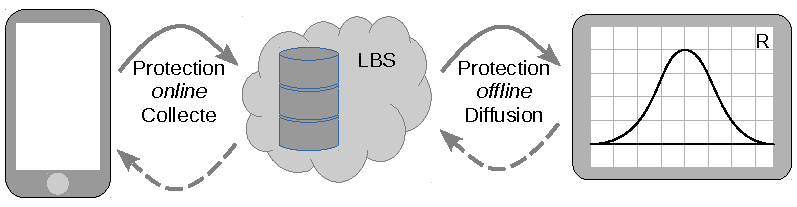
\includegraphics[scale=0.78]{Schema_phases.pdf}
\end{center} 
Les mécanismes de protection opéreront sur l'une ou l'autre et dépendent des cas d'utilisation, qu'on classe en plusieurs catégories: le \textbf{temps réel}, où l'utilisateur a besoin d'une réponse quasi-immédiate, ce qui impose des contraintes fortes en termes de débit et d'efficacité du traitement. 
L'utilisation \textbf{hors ligne}, avec des données collectées dans un premier temps, puis publiées par la suite pour analyse, comme dans le cas du mouvement \emph{open data}, ou pour alimenter les algorithmes d'apprentissage automatique. 
Enfin, le \textbf{traitement par lots} envoyés à intervalles réguliers de l'utilisateur au LBS, qui constitue un mode intermédiaire. 
%% + Schéma user / LBS / Data analyst p2
\VESP

Plusieurs types de métriques devront être définies pour évaluer l'efficacité de ces mécanismes, dans les domaines suivants:\nopagebreak
\begin{itemize}
    \item 
    \textbf{Confidentialité}: quel en est le niveau garanti face aux attaques envisageables?
    \item %% ou Exploitabilité ??
    \textbf{Utilisabilité\footnote{Il n'est pas évident de traduire \og \emph{utility}\fg{} dans ce cadre. \og Utilité\fg{} nous paraissait insuffisamment explicite; nous avons également pensé à \og exploitabilité\fg{}. Il s'agit d'évaluer la préservation d'un contenu suffisamment utilisable dans les données traitées par un mécanisme de protection, autrement dit leur pertinence résiduelle.}}: ce point fera l'objet d'un nécessaire compromis avec le précédent. En effet, on imagine aisément les cas extrêmes: fournir la ressource telle quelle, sans dégradation mais sans aucune protection, ou à l'opposé ne rien divulguer, ce qui lui ôte tout intérêt.
    \item 
    \textbf{Performance}: le temps d'exécution (crucial en temps réel), la scalabilité (notamment pour la partie \emph{offline}), la tolérance aux pannes sont plus ou moins importants selon le contexte. Ces aspects restent indépendants des deux précédents. Ils seront moins pris en compte dans la suite.
    \end{itemize}

Les illustrations suivantes sont essentiellement tirées de l'enquête de Vincent Primault \textit{et al}. publiée en $2\,019$~\cite{PBMB19}, qui prend en compte ces trois critères. Nous renvoyons à cette publication pour les références et résultats chiffrés précis.
%
\subsection{Exemples d'exploitation de données de localisation}
Différentes expérimentations fournissent des exemples qui permettent de se donner une meilleure représentation de la menace, dans ce contexte particulier.
\begin{itemize}
    \item 
    Identification de \og \textbf{point d'intérêt}\fg{}: à partir de traces de localisation, on peut déterminer des lieux ou moments particuliers, porteurs d'une sémantique forte. 
    Par exemple à partir de traces GPS de taxis, indiquant notamment les pauses, on a pu retrouver des adresses personnelles ou repérer les périodes de prières indiquant des chauffeurs musulmans avec une certaine probabilité.
    Avec l'évolution rapide des performances en apprentissage automatique, la découverte de tels points particuliers est facilité.
    \item 
    Mise en évidence de \textbf{relations sociales}: en analysant les proximités temporelle et géographiques, avec des seuils bien choisis, des liens probables entre individus peuvent être établis. 
    En y ajoutant la sémantique des lieux de rencontre, on parvient alors à caractériser ces relations sociales. 
    Un arbre de décision peut être établi, pour classer par catégories avec une bonne probabilité.
    \item 
    \textbf{Ré-identification}: on arrive même à déterminer l'identité d'un utilisateur dans certains cas à partir de ses traces de localisation. 
    En effet, elles sont relativement uniques pour chaque individu: 4 points spatiaux-temporels aléatoires sont généralement suffisants pour caractériser une personne dans une foule. 
    Le simple couple (lieu de travail; habitation), ne serait-ce qu'indiqué à l'échelle du \og bloc\fg{}, est déjà fortement discriminant, alors qu'en réalité les données temporelles s'avèrent aussi importantes que la localisation géographique.
    Et même quand le graphe sous-jacent est vidé de ses données (celui des 10 lieux les plus fréquentés par exemple), sa topologie permet encore de retrouver une majorité d'individus!\\
    Ajoutons que le matériel utilisé et les paramètres logiciels suffisent généralement déjà à fabriquer un profil unique\footnote{Voir \url{https://amiunique.org/fp} en ce qui concerne la navigation sur le web.} et que les appareils connectés sont richement dotés en capteurs divers\footnote{\url{https://epu2017.sciencesconf.org/data/Delabre.pdf} le détaille en pages 5-6.}, potentiellement bavards. La combinaison de ces informations est donc redoutable.
    \item 
    \textbf{Prédiction de mobilité}: modéliser les habitudes permet à des algorithmes d'apprentissage automatique de prédire un prochain lieu de présence, par exemple sur des points de \emph{check-in} de Fourquare ---~dont la devise actuelle en page d'accueil est: \emph{\og "où" est la clé\fg{}}\footnote{\url{https://fr.foursquare.com/}}. 
    Certaines études montrent la possibilité de prévisions à plus longue échéance, en termes de lieu et créneau horaire. 
\end{itemize}
Si ces exemples devraient suffire à se convaincre qu'il faut se préoccuper sérieusement de la protection de ce type de données, encore faut-il définir clairement ce qu'on entend par là. 
C'est indispensable pour évaluer les mécanismes mis en œuvre et les éventuels risques pris. 
Par ailleurs, décrire à l'utilisateur les garanties qui lui sont offertes nécessite également des concepts explicites, accessibles sans connaissances techniques avancées.
%% ========================================================================================== %%
%%
\section{Modélisation de la confidentialité}
%%
Les données individuelles sensibles ne se limitent pas au domaine de la localisation. Ainsi, dans cette partie on se place fréquemment dans un cadre plus large.
%
\subsection{Échec des approches naïves}
%
Pour la première fois, en $\mathbf{1\,977}$, le statisticien suédois \textbf{Tore Dalenius} définit précisément une garantie de confidentialité\cite{D77}: en accédant à une base de données, l'adversaire ne doit pas être capable d'obtenir une information nouvelle sur un individu, qui ne pourrait être apprise sans y accéder. 
Cynthia Dwork montrera que ce Graal reste inaccessible, notamment à cause de potentielles informations auxiliaires comme on l'a vu sur divers exemples, ce qui a motivé la mise au point d'autres concepts moins rigides.

La question de la protection des caractéristiques individuelles sensibles quand on stocke ou qu'on diffuse des données à des fins d'analyse globale s'est posée bien avant la vague de l'\emph{open data} et le boom de l'apprentissage automatique (le premier recensement américain date de $1\,790$ par exemple).
Pour permettre des statistiques sur les habitants d'un état ou d'une région, il est tentant de fournir la base des données dans laquelle on a substitué des numéros aléatoires aux véritables noms (\emph{par exemple en \og hachant\fg{} ces derniers}) afin de gommer les identités réelles inutiles pour l'étude. 
Mais cette démarche dite de \textbf{pseudonymisation}, comme son nom l'indique, s'avère incapable de garantir l'anonymat et il reste souvent possible de retrouver un bon nombre, voire toutes les identités des individus enregistrés dans la base.

En effet, si un bon aléa ou un hachage robuste permettent en principe d'empêcher de retrouver les noms réels à partir des pseudonymes, c'est sans compter avec le recours à des bases d'informations auxiliaires: la faille tient aux données elles-mêmes, dont on peut retrouver une partie par ailleurs afin de les ré-associer à un individu. 
On qualifie de \textbf{quasi-identifiant} ces $n$-uplets de champs présents dans des enregistrements d'une base et qui caractérisent chacun d'entre eux, au moins avec une forte probabilité. 
Par exemple dans une table de patients hospitalisées, où la pathologie traitée constitue une information sensible, la donnée (âge approximatif; poids approximatif; origine ethnique; statut marital) permet d'identifier des malades de manière quasi-unique~\cite{DN03}. On a déjà largement montré également dans la partie précédente que certaines données de localisation jouaient clairement ce rôle.

Plusieurs affaires classiques l'ont également parfaitement illustré en situation réelle. Ainsi, en $2\,006$, \textbf{AOL} publie\footnote{Détails sur \url{https://www.nytimes.com/2006/08/09/technology/09aol.html}} quelques $20$ millions de recherches effectuées par plus de $650\,000$ de ses utilisateurs, après avoir \emph{remplacé} les noms par des nombres aléatoires (afin d'étudier des liens éventuels entre les différentes recherches d'une personne, ce qu'une simple \emph{suppression} des identités ne permettrait pas). Or, certains citoyens ont pu être ré-identifiés (adresses, numéros de sécurité sociale, noms). En effet, nos recherches constituent souvent une \og empreinte digitale\footnote{Nous ne réitérerons pas ce jeu de mot, exploitant la traduction courante de \og \emph{digital}\fg{} par un adjectif qualifiant en principe ce qui a trait aux doigts plutôt que par \og numérique\fg{}, mais notons qu'ici les deux acceptions concordent de manière cocasse.}\fg{} unique. 

Un autre cas marquant est celui de \textbf{Netflix}, qui diffuse en octobre de la même année $2\,006$ les recommandations pseudonymisées de $500\,000$ clients. Au départ, il s'agit un prix d'un million de dollars à décerner au meilleur algorithme de recommandation. Mais Arvind Narayanan et Vitaly Shmatikov de l'université d'Austin au Texas ont montré~\cite{ANVS06} qu'ils pouvaient ré-identifier plusieurs profils, en exploitant notamment des données IMDB (\emph{Internet Movie Database}). Cela vaudra une \emph{class action} à Netflix\footnote{Voir \url{https://en.wikipedia.org/wiki/Netflix\_Prize\#Privacy\_concerns}} et un règlement amiable sans doute coûteux, ce qui rappelle au passage l'importance du respect de la sphère privée au delà de tout aspect éthique.

Ces différents exemples démontrent clairement que \textbf{la pseudonymisation est totalement insuffisante}. Ils ont également l'intérêt de rappeler qu'on ne peut pas se fier à la seule intuition:  \textbf{une protection rigoureusement démontrée est nécessaire} et elle doit tenir compte de potentielles connaissances auxiliaires de l'adversaire, externes à la base sensible et par nature impossibles à borner.
%
\subsection{$k$-anonymat et notions connexes}
%
Cette parade à la ré-identification se base sur l'agrégation de données, déjà en usage en statistiques. 
\textbf{Latanya Sweeny} de l'université d'Harvard l'a introduite en $\mathbf{2\,002}$~\cite{S02} après une participation à une publication sur ce thème en $1\,998$~\cite{SS98}, dans des articles où elle définit la notion de quasi-identifiant.

Sans rentrer dans un formalisme inutile ici, le $k$-anonymat (pour $k\in\mathbb{N}^*$) est la \textbf{garantie qu'un quasi-identifiant} quelconque \textbf{est associé à $k$ enregistrement} de la base \textbf{au minimum}, donc qu' individu est protégé au sein d'un \og groupe d'anonymat\fg{} d'effectif $k$ ou plus.
La probabilité d'identification individuelle tomberait donc à $\frac{1}{k}$ dans le pire des cas. 

Concrètement, on doit d'abord identifier les regroupements d'attributs non sensibles susceptibles d'identifier une ligne de la base.
Ensuite, on réduit le niveau de détail des valeurs de certains champs, jusqu'à pouvoir garantir qu'à chaque quasi-identifiant sont associés au moins $k$ enregistrements: on peut regrouper des données numériques en classes, agréger des catégories. C'est la phase de généralisation. Prenons un exemple avec $k=2$:
%GARDER?
\begin{center}
    \small\sffamily
\begin{tabular}{|c|c|c|c|}
    \hline 
    \textbf{Nom} & \textbf{Âge} & \textbf{CP} & \textbf{Traitement} \\ 
    \hline \hline
    $\cdots$ & 19 & 25\,000$_\text{B}$ & Asthme \\ 
    \hline 
    $\cdots$ & 43 & 25\,200$_\text{M}$ & Cancer \\ 
    \hline 
    $\cdots$ & 73 & 25\,170$_\text{B}$ & Leucémie \\ 
    \hline 
    $\cdots$ & 27 & 25\,480$_\text{B}$ & VIH \\ 
    \hline 
    $\cdots$ & 35 & 25\,120$_\text{M}$ & VIH \\ 
    \hline 
    $\cdots$ & 61 & 25\,000$_\text{B}$ & Leucémie \\ 
    \hline 
\end{tabular} 
$\Rightarrow$
\begin{tabular}{|c|c|c|}
    \hline 
    \textbf{Âge} & \textbf{Arrond.} & \textbf{Traitement} \\ 
    \hline \hline
    18-30 & Besançon & Asthme \\ 
    \hline 
    18-30 & Besançon & VIH \\ 
    \hline \hline
    35-45 & Montbéliard & Cancer \\ 
    \hline 
    35-45 & Montbéliard & VIH \\ 
    \hline \hline
    \emph{60+} & \emph{Besançon} & \emph{Leucémie} \\ 
    \hline 
    \emph{60+} & \emph{Besançon} & \emph{Leucémie} \\ 
    \hline 
\end{tabular}
\end{center}
Cependant, des failles subsistent: à partir d'un quasi-identifiant, il reste souvent possible de savoir que certaines valeurs sont exclues, pour un champ sensible (asthme impossible pour \og 35-45, Montbéliard\fg{}), ou que d'autres sont plus probables que dans la population globale.
Et en cas de valeur identique sur des données sensibles pour tous les membres d'un groupe d'anonymat, on retrouve même cette information de manière certaine (\emph{leucémie, pour \og 60+, Besançon\fg{}}).

Pour éviter cette situation, le concept de $\ell$-diversité ajoute la contrainte que tout groupe d'anonymat contienne au minimum $\ell$ valeurs distinctes des données sensibles à protéger. 
Pour accentuer l'indiscernabilité, on utilise parfois en plus la $t$-proximité: la distribution de chaque valeur sensible dans tout groupe d'anonymat doit alors rester suffisamment proche de celle observée dans la population globale. Dans ce dernier cas, on risque cependant de perdre l'intérêt même de l'étude des données, en gommant trop les corrélations...

L'un de ses intérêt majeurs du $k$-anonymat est qu'il est \textbf{compréhensible par un non-spécialiste, l'utilisateur} d'un LBS en ce qui nous concerne.
Or précisément, dans un cadre idéal en tout cas, c'est lui qui devra accepter ou non de céder ses données, suivant les garanties qu'on lui fournit et qu'il doit donc cerner correctement.
Cependant, ce concept n'est pas toujours simple à mettre en œuvre, à automatiser. Et on l'a vu, des failles peuvent subsister. 
%
\subsection{Confidentialité différentielle}
%
En $\mathbf{2\,006}$, \textbf{Cynthia Dwork} chercheuse chez Microsoft publie un article qui reste une référence, sur le concept de confidentialité différentielle. 
Sa richesse tient à son approche formelle, aux démonstrations des propriétés garanties indépendamment de toute connaissance \textit{a priori} de l'adversaire.
Partant du constat que toute publication même mineure transgresse la définition de Dalenius, elle travaille sur la quantification de l'information potentiellement divulguée.
Elle propose alors un mécanisme qui transforme les valeurs sensibles véridiques, afin que le résultat reste exploitable de manière statistique dans sa globalité, tout en préservant au mieux les informations individuelles.
%Un compromis entre le niveau de perte de confidentialité et l'utilisabilité de la transcription des données s'avère incontournable.

Notons que le nom lui-même s'inspire de la dérivation ou de la différenciation: on s'intéresse à la variation de la réponse à une requête, pour une petite modification de la base.

\subsubsection{Aux origines: les réponses \og randomisées\fg{}}
L'une des idées fondatrices est l'utilisation des réponses randomisées: ce mécanisme de protection introduit une part d'aléa entre la valeur réelle et celle qui est consignée ou diffusée.
L'exemple de référence, d'ailleurs repris dans la présentation de RAPPOR~\cite{EPK14}, est l'utilisation de ce concept lors d'un sondage sur une question embarrassante (à propos de croyances, d'appartenance politique, de pratiques répréhensibles, etc.), pour laquelle on veut éviter que le sondé mente par crainte de se dévoiler. 
On le doit à \textbf{Stanley L. Warner} ($\mathbf{1\,965}$)~\cite{W65}.

En voici tout d'abord une version simplifiée.
Considérons que c'est la réponse \og Oui\fg{} qui peut être gênante. 
On demande à la personne interrogée de tirer secrètement à \og Pile ou Face\fg{}: si elle tombe sur \og Pile \fg{}, elle doit répondre de manière honnête, sinon elle doit choisir le \og Oui\fg{}.
D'une part, cela lui garantit un \textbf{déni plausible}, concept clé dans ce cadre: rien ne permet d'être certain qu'une réponse \og Oui\fg{} correspond à la réalité.
D'autre part, on peut toujours estimer à partir du sondage la proportion $p$ réelle de la caractéristique embarrassante à partir du taux $r\approx\mathbb{P}(\text{\og{}Oui\fg{}})$ des réponses affirmatives (on montre aisément que $p\approx2r-1$).
% Arbre
\begin{center}
    \begin{tikzpicture}[scale=0.7]
    % Styles (MODIFIABLES)
    \tikzstyle{fleche}=[->,>=latex,thick]
    \tikzstyle{noeud}=[]%fill=yellow,circle,draw
    \tikzstyle{feuille}=[right]%[fill=yellow,circle,draw]
    \tikzstyle{etiquette}=[midway]%[midway,fill=white,draw]
    % Dimensions (MODIFIABLES)
    \def\DistanceInterNiveaux{3}
    \def\DistanceInterFeuilles{1}
    % Dimensions calculées (NON MODIFIABLES)
    \def\NiveauA{(0)*\DistanceInterNiveaux}
    \def\NiveauB{(1.5)*\DistanceInterNiveaux}
    \def\NiveauC{(2.5)*\DistanceInterNiveaux}
    \def\InterFeuilles{(-1)*\DistanceInterFeuilles}
    % Noeuds (MODIFIABLES : Styles et Coefficients d'InterFeuilles)
    \node[noeud] (R) at ({\NiveauA},{(1.25)*\InterFeuilles}) {};
    \node[noeud] (Ra) at ({\NiveauB},{(0.5)*\InterFeuilles}) {Pile};
    \node[feuille] (Raa) at ({\NiveauC},{(0)*\InterFeuilles}) {Oui$\qquad p/2$};
    \node[feuille] (Rab) at ({\NiveauC},{(1)*\InterFeuilles}) {Non$\qquad (1-p)/2$};
    \node[noeud] (Rb) at ({\NiveauB},{(2)*\InterFeuilles}) {Face};
    \node[feuille] (Rba) at ({\NiveauC},{(2)*\InterFeuilles}) {Oui$\qquad 1/2$};
    % Arcs (MODIFIABLES : Styles)
    \draw[fleche] (R)--(Ra) node[etiquette, above] {\footnotesize$1/2$};
    \draw[fleche] (Ra)--(Raa) node[etiquette, above] {\footnotesize$p$};
    \draw[fleche] (Ra)--(Rab) node[etiquette, below] {\footnotesize$1-p$};
    \draw[fleche] (R)--(Rb) node[etiquette, below] {\footnotesize$1/2$};
    \draw[fleche] (Rb)--(Rba);
    \end{tikzpicture}
\end{center}
On peut objecter que le déni plausible n'est pas accordé à la réponse \og Non\fg{}, ce qui pourrait pousser à fournir cette dernière de manière malhonnête, pour s'assurer une solide couverture. 
On peut donc proposer le raffinement suivant, le principe essentiel restant le même: le sondé tire deux fois à \og Pile ou Face\fg{}. S'il obtient \og Pile \fg{} la première fois, il répond de manière honnête, sinon, c'est le second tirage qui décide du résultat: \og Oui\fg{} pour \og Pile\fg{}, ou alors \og Non\fg{}. 
Les deux valeurs peuvent alors être mise en doute et l'on peut toujours estimer les véritables proportions dans le groupe sondé ($p\approx2r-\frac{1}{2}$).
% ****** idem : arbre, calcul ?
\begin{center}
    % Racine à Gauche, développement vers la droite
    \begin{tikzpicture}[scale=0.7]
    % Styles (MODIFIABLES)
    \tikzstyle{fleche}=[->,>=latex,thick]
    \tikzstyle{noeud}=[]%fill=yellow,circle,draw
    \tikzstyle{feuille}=[right]%[fill=yellow,circle,draw]
    \tikzstyle{etiquette}=[midway]%[midway,fill=white,draw]
    % Dimensions (MODIFIABLES)
    \def\DistanceInterNiveaux{3}
    \def\DistanceInterFeuilles{1}
    % Dimensions calculées (NON MODIFIABLES)
    \def\NiveauA{(0)*\DistanceInterNiveaux}
    \def\NiveauB{(1.5)*\DistanceInterNiveaux}
    \def\NiveauC{(2.5)*\DistanceInterNiveaux}
    \def\InterFeuilles{(-1)*\DistanceInterFeuilles}
    % Noeuds (MODIFIABLES : Styles et Coefficients d'InterFeuilles)
    \node[noeud] (R) at ({\NiveauA},{(1.5)*\InterFeuilles}) {};
    \node[noeud] (Ra) at ({\NiveauB},{(0.5)*\InterFeuilles}) {Pile};
    \node[feuille] (Raa) at ({\NiveauC},{(0)*\InterFeuilles}) {Oui$\qquad p/2$};
    \node[feuille] (Rab) at ({\NiveauC},{(1)*\InterFeuilles}) {Non$\qquad (1-p)/2$};
    \node[noeud] (Rb) at ({\NiveauB},{(2.5)*\InterFeuilles}) {Face};
    \node[feuille] (Rba) at ({\NiveauC},{(2)*\InterFeuilles}) {Oui$\qquad 1/4$};
    \node[feuille] (Rbb) at ({\NiveauC},{(3)*\InterFeuilles}) {Non$\qquad 1/4$};
    % Arcs (MODIFIABLES : Styles)
    \draw[fleche] (R)--(Ra) node[etiquette, above] {\footnotesize$1/2$};
    \draw[fleche] (Ra)--(Raa) node[etiquette, above] {\small$p$};
    \draw[fleche] (Ra)--(Rab) node[etiquette, below] {\footnotesize$1-p$};
    \draw[fleche] (R)--(Rb) node[etiquette, below] {\footnotesize$1/2$};
    \draw[fleche] (Rb)--(Rba) node[etiquette, above] {\footnotesize$1/2$ \tiny (Pile)};
    \draw[fleche] (Rb)--(Rbb) node[etiquette, below] {\footnotesize$1/2$ \tiny (Face)};
    \end{tikzpicture}
\end{center}
En fait, Warner fournit même une autre version, avec un tirage aléatoire non équiprobable, dans lequel dans un cas on pose la question \og avez vous la caractéristique C ?\fg{} et dans l'autre la question contraire \og est-il vrai que vous ne possédez pas la caractéristique C ?\fg{}
%%% **** résultats ? schéma ??

En $2\,015$ Graeme BLAIR, Kosuke IMAI et Yang-Yang ZHOU de l'université de Princeton ont recensé les applications pratiques de ce concept et ont créé des outils permettant notamment des prédictions, comme avec les modèles de régression~\cite{BIZ15}.

Malheureusement, nous allons voir que ces réponses randomisées à elles seules restent insuffisantes.
%
\subsubsection{Les limites des perturbations aléatoires}
%
Si la protection est solide pour une interrogation \emph{unique} d'une personne donnée, elle s'amenuise clairement si on la réitère, dans le cadre d'un relevé quotidien par exemple. 
En effet, une analyse statistique permettra alors d'approcher la valeur réelle individuelle.

D'un point de vue formel, \textbf{Irit Dinur et Kobbi Nissim} on montré en $\mathbf{2\,003}$~\cite{DN03} que l'ajout d'un bruit important aux données d'une base était nécessaire pour garantir un minimum de confidentialité. 
En pratique, un tel bruit ruine la pertinence des requêtes.
Plus précisément, en considérant une base assimilée à une chaîne de $n$ bits, l'ajout d'une perturbation en $\Omega(\sqrt{n})$ est nécessaire, sans quoi un adversaire peut en reconstruire en temps polynomial une très bonne approximation, à partir de requêtes renvoyant des sommes de bits (bruitées) sur un ensemble de positions bien choisies. 
La preuve repose sur un algorithme où ces sommes sont vues comme des codes correcteurs, qui utilise la programmation linéaire.
Si l'adversaire n'est pas limité dans ses requêtes, le bruit doit même être linéaire en $n$ pour assurer une garantie suffisante.

Dès lors, puisque la protection parfaite est illusoire si l'on veut tirer partie des données, le besoin de quantification de ce qui est potentiellement divulgué devient primordial.
%
\subsubsection{$\epsilon$-indiscernabilité, pour $\epsilon>0$}% EPK14
%% BUT en 1er, non formel
Cynthia Dwork ---~qui avait déjà œuvré aux côtés de Dinur et Nissim concernant l'article précédemment cité~---, Frank McSherry, Kobbi Nissim et Adam D. Smith en donnent la définition, dans cet article de $2\,006$\cite{DMNS06} qui leur vaudra le prix Gödel $2\,017$\footnote{\url{http://eatcs.org/index.php/component/content/article/1-news/2450-2017-godel-prize}}.
Ce concept s'applique à un mécanisme de réponse randomisée qu'on notera $\tau$, opérant sur des bases de données ($\tau$ renvoie à partir d'une requête la somme de la réponse véritable et d'un \og bruit\fg{} bien choisi). 
L'idée est de garantir que deux bases proches sont associées à des images par $\tau$ suffisamment semblables. 
De manière originale, on s'intéresse donc ici à la \textbf{confidentialité en fonction du mécanisme} d'interrogation de la base. 

\emph{Définition}: un \textbf{mécanisme $\mathbf{\tau}$ est $\mathbf{\epsilon}$-indiscernable} si, pour toutes bases $\mathtt{x}$ et $\mathtt{x'}$ qui diffèrent exactement d'une entrée, pour toute réponse $t$ appartenant à l'image de $\tau$ et pour tout adversaire (\emph{qui pourrait intervenir dans le choix des requêtes}), on a:
\[\left|\ln\left(\frac{\mathbb{P}(\tau(\mathtt{x})=t)}{\mathbb{P}(\tau(\mathtt{x'})=t)}\right)\right|\leqslant\epsilon\]
Cela se traduit \emph{approximativement}, pour les petites valeurs de $\epsilon$ et en tenant compte du fait qu'on a alors $\exp(\epsilon)\approx1+\epsilon$, par
\[\frac{\mathbb{P}(\tau(\mathtt{x})=t)}{\mathbb{P}(\tau(\mathtt{x'})=t)} \in \left[1-\epsilon \text{ ; } 1+\epsilon \right]\]
soit, compte tenu des rôles symétriques de $\mathtt{x}$ et $\mathtt{x'}$, par
\[\mathbb{P}\left(\tau(\mathtt{x})=t\right) \leqslant (1+\epsilon)\cdot\mathbb{P}\left(\tau(\mathtt{x'})=t\right)\]
Plus formellement, une base $\mathtt{x}\in D^n$ est un vecteur de $n$ entrées d'un domaine $D$ qui vaut $\left\{0;1\right\}^d$ ou $\mathbb{R}^d$; $\tau$ est une variable aléatoire sur $D^n$ et $t\in\tau(D^n)$. Remarquons que le nombre d'entrées qui diffèrent entre deux bases $\mathtt{x}$ et $\mathtt{x'}$ est la distance de Hamming sur $D^n$, qu'on notera  $d_H(\mathtt{x},\mathtt{x'})$.

\vspace{0.6em}

Illustrons cette notion à l'aide de cas particuliers.
\begin{itemize}
    \item 
    \textbf{Sondage randomisé}: reprenons l'exemple initial avec une réponse en \og Oui\fg{} / \og Non\fg{}, où un premier lancer aléatoire détermine de manière équiprobable si l'on doit répondre honnêtement, ou en se basant sur le résultat d'un second lancer. Si la réalité se traduit par \og Oui\fg{}, la réponse affirmative sera donnée avec une probabilité de $\frac{3}{4}$; dans le cas contraire, cette proportion est de $\frac{1}{4}$. La situation est symétrique quand la caractéristique réelle est opposée. On en déduit qu'entre deux données véridiques contraires (\emph{deux bases $\mathtt{x}$, $\mathtt{x'}$ réduites à un enregistrement avec $d_H(\mathtt{x},\mathtt{x'})=1$}), on a si l'on note $\tau$ ce mécanisme de sondage et si $t$ vaut \og Oui\fg{} ou \og Non\fg{},
    \[\left|\ln\left(\frac{\mathbb{P}(\tau(\mathtt{x})=t)}{\mathbb{P}(\tau(\mathtt{x'})=t)}\right)\right| 
    \leqslant
    \ln \left( \frac{3/4}{1/4} \right)
    = \ln 3\]
    Ce sondage randomisé est donc $\epsilon$-indiscernable avec $\epsilon=\ln 3$.    
    \item 
    \textbf {Sommes bruitées}: on considère une base $\mathtt{x}\in\{0,1\}^n$, donc réduite à $n$ enregistrements valant $0$ ou $1$. On souhaite en extraire le nombre de $1$, à savoir $f(\mathtt{x})=\sum_i{x_i}$. On définit le mécanisme $\tau$ par $\tau=f+Y$, où $Y$ est une variable aléatoire qui suit la loi de Laplace $Lap(1/\epsilon)$, de densité proportionnelle à $h(y)=\exp(-\epsilon|y|)$. 
    
    Celui-ci est alors $\epsilon$-indiscernable: en effet, comme $|y'|-|y|\leqslant|y'-y|$,\\ $\frac{h(y)}{h(y')}\leqslant\exp\left(\epsilon|y'-y|\right)$. De plus: $\tau(\mathtt{x})=t \Leftrightarrow Y = t-f(\mathtt{x})$.
    Donc (en s'autorisant un abus de notation entre distributions discrètes et continue)  $\frac{\mathbb{P}\left(\tau(\mathtt{x})=t\right)}{\mathbb{P}\left(\tau(\mathtt{x'})=t\right)}=
    \frac{h\left(t-f(\mathtt{x})\right)}{h\left(t-f(\mathtt{x'})\right)}\leqslant\mathrm{e}^{\left(\epsilon|f(\mathtt{x})-f(\mathtt{x'}|)\right)}\leqslant\mathrm{e}^{\epsilon}$, 
    si $d_H(\mathtt{x},\mathtt{x'})=1$.\\[0.2em]
    \emph{Nous reviendrons sur le choix de la loi et du paramètre pour $Y$}.
    \item 
    \textbf{Contre-exemple}: l'$\epsilon$-indiscernabilité peut s'avérer impossible pour certaines fonctions de requête, quel que soit le mécanisme associé:
    En considérant $f(\mathtt{x})=\max_i(x_i)$ pour une base $\mathtt{x}$ de \textit{n} réels, en modifiant par exemple $x_1$ dans $\mathtt{x}$, on peut obtenir deux bases Hamming-distantes de $1$ telles que les images par $f$ soient arbitrairement éloignées, donc des mécanismes randomisés associés subiront le même sort. Une valeur
    image par un tel mécanisme peut donc avoir une probabilité nulle sur l'une des bases et non nulle sur l'autre, rendant le quotient des probabilités de la définition infini.
\end{itemize}

Cette notion d'$\epsilon$-indiscernabilité est plus contraignante que la \og proximité statistique\fg{} utilisée en cryptographie, puisqu'on peut créer deux bases arbitrairement proches d'un point de vue statistique, mais dont le ratio des probabilités dans la formule est infini, en fixant comme on vient de le voir la probabilité d'une valeur dans une série à zéro et pas dans l'autre.
Malgré tout, on verra qu'on peut souvent l'atteindre à un coût relativement faible. De plus, elle a des formulations plus \og sémantiques\fg{}, moins formelles, donc elle correspond à ce qu'on attend d'elle.

Son originalité est de considérer la situation \textbf{en fonction de la requête} $f$ envisagée. Reste à savoir comment choisir le bruit $Y$ pour obtenir une $\epsilon$-indiscerna\-bilité optimale pour $\tau=f+Y$.
%
\subsubsection{Sensibilité d'une fonction de requête}
%
Dwork cherche alors à caractériser les fonctions définies sur l'ensemble des bases $D^n$, de manière à pouvoir déterminer la perturbation ajoutée pour obtenir un mécanisme $\tau$ qui soit $\epsilon$-indiscernable.

La \textbf{${L_1}$-sensibilité} d'une fonction $f: D^n\rightarrow\mathbb{R}^d$ est le plus petit réel \textbf{$S(f)$} tel que, pour toute base $\mathtt{x}$ et toute base $\mathtt{x'}$ dans $D^n$ avec $d_H(\mathtt{x},\mathtt{x'})=1$,
\[\left\| f(\mathtt{x})-f(\mathtt{x'})\right\|_1\leqslant S(f)\]
On omet en général le $L_1$ et c'est ce que nous ferons dans la suite, bien qu'on puisse travailler de manière analogue avec d'autres normes.\\[-0.4em]

Un point essentiel: cette notion est une \textbf{propriété intrinsèque de $f$}, indépendante de la base de donnée sur laquelle elle opère. 
C'est ce qui va permettre de calibrer le bruit ajouté et donc le mécanisme global uniquement à partir de la requête $f$ envisagée. 
Dès lors, interroger une base complète se fera sans perte de confidentialité par rapport à une demande identique sur un échantillon restreint.\\[-0.4em]

Reprenons quelques exemples:
\begin{itemize}
    \item 
    \textbf{Sommes bruitées}: sur $\mathtt{x}\in\{0,1\}^n$, on rappelle qu'on cherche à extraire $f(\mathtt{x})=\sum_i{x_i}$. La modification d'un enregistrement $x_i$ d'une base à une autre peut modifier au maximum de $1$ la valeur de  $f(\mathtt{x})$, d'où une sensibilité $S(f)=1$.
    \item 
    \textbf{Histogrammes}: le domaine $D$ est partitionné en $d$ parties $B_1,\,\ldots\,, B_d$. On considère la fonction $f:D^n\longrightarrow\mathbb{N}^d$ où chaque coordonnée de l'image, de $k=1$ à $k=d$, indique le nombre de valeurs dans $B_k$. Changer l'une des valeurs de $D$ dans la base peut modifier au plus $2$ coordonnées de son image (\emph{une augmente de 1, une autre diminue d'autant, si la nouvelle valeur de départ n'appartient plus à la même catégorie}): puisque la norme considérée est $L_1$, on en déduit $S(f)=2$.
\end{itemize}

Cette notion de sensibilité va prendre tout son sens en permettant de régler finement la perturbation aléatoire en fonction du type de requête, de manière à obtenir l'$\epsilon$-indiscernabilité.
%
\subsubsection{Calibrage du bruit: mécanisme de Laplace}%étalonnage ?
%
En raisonnant comme précédemment dans le cas des sommes bruitées, en remarquant qu'un vecteur dont les coordonnées sont indépendantes et identiquement distribuées suivant $Lap(\lambda)$ suit une loi de densité proportionnelle à $f(\nu)=\exp(-\|\nu\|_1/\lambda)$, on montre le résultat suivant:\\[-0.4em]

\emph{Théorème}: Pour tout réel $\epsilon>0$ et toute fonction $f:D\longrightarrow\mathbb{R}^n$ de sensibilité $S(f)$, on définit  $\tau:D\longrightarrow\mathbb{R}^n$ par $\tau=f+Y$, où $Y$ est une variable aléatoire qui suit la loi de Laplace centrée $Lap\left(S(f)/\epsilon\right)$\footnote{Dans $\mathbb{R}$, la loi de Laplace (ou \og double exponentielle\fg{}) centrée $Lap(\lambda)$ a comme densité $f(\nu)=\frac{1}{2\lambda}\exp(-\frac{| \nu|}{\lambda})$. On l'étend ici à $\mathbb{R}^d$ avec des composantes indépendantes et identiquement distribuées selon cette loi dans $\mathbb{R}$.}.\\
Le mécanisme $\tau$ est alors $\epsilon$-indiscernable.\\[-0.4em]
% **** idée de la démo 

L'exemple des sommes bruitées n'était qu'un cas particulier: on avait $S(f)=1$, d'où le choix d'un bruit laplacien $Y$ de paramètre $S(f)/\epsilon = 1/\epsilon$.

De même, on peut reprendre le contre-exemple précédent, où l'on étudie $f(\mathtt{x})=\max_i(x_i)$ pour une base $\mathtt{x}$ de \textit{n} réels. Ici, la sensibilité est infinie, donc le théorème ne s'applique pas (\emph{et on avait déjà montré qu'en effet, l'$\epsilon$-indiscernabilité n'était pas envisageable}).\\[-0.4em]

Ce résultat se généralise à des requêtes successives sur une base, potentiellement construites en fonction des réponses aux précédentes dans un \textbf{processus adaptatif}.
Une requête y est alors dépendante des précédentes ainsi que des valeurs de retour.
On notera $t$ cette séquence de questions-réponses. La requête $Q_i$ est donc fonction des valeurs $t_1$, ..., $t_{i-1}$.

\emph{Théorème}: on note $f_t(\mathtt{x}): D^n\longrightarrow\mathbb{R}^d$ la requête paramétrée par la transcription $t$, dont la $i$-ème coordonnée est associée à la $i$-ème requête.\\ 
Si $\lambda = \max_t S(f_t)/\epsilon$, alors le mécanisme  est $\epsilon$-indiscernable.\\[-0.4em]

% Justif. rapide (p9 ?)

Exemples de fonctions à faible sensibilité, dont l'intérêt réside dans le peu de bruit à ajouter pour assurer la confidentialité différentielle:
\begin{itemize}
    \item 
    \textbf{Histogrammes}: on a montré que $S(f)=2$ pour la fonction $f$ qui renvoie le vecteur des effectifs des enregistrements dans chacune des parties $B_1$ à $B_d$, d'où un bruit indépendant de $d$ alors qu'il était $k$ fois supérieur pour $k\in O(\sqrt{d})$ en s'en tenant à un résultat établi précédemment~\cite{BDMK05} % sur les requêtes sublinéaires
    \item 
    \textbf{Analyse disjointe}: au delà de ce simple décompte, on peut généraliser le résultat à toute analyse renvoyant la valeur image par une fonction $f$ de chaque partie $B_i$, notée $f(\mathtt{x})_i$. 
    On montre alors que $S(f)\leqslant2\max_i\,S\left(f(\mathtt{x})_i\right)$, toujours indépendamment de $d$.
    \item 
    \textbf{Vecteur moyen et matrice de covariance}: pour une fonction $v:D\longrightarrow\mathbb{R}^d$ où $D$ comporte $n$ enregistrements, si dans $\mathbb{R}^d$,  $\mu$ renvoie le vecteur des moyennes des $n$ composantes et $C$ leur matrice de covariance et si l'on note $\gamma=\max_x\left\|v(x)\right\|_1$, on montre que $S(\mu)\leqslant2\gamma/n$ et que $S(C)\leqslant 8\gamma^2/n$.
    C'est $k$ fois mieux que ce qu'en première analyse, avec $k\in O(d)$.
    \item 
    \textbf{Distance par rapport à une propriété}: en notant $\delta_S$ la distance à un ensemble $S\subseteq D^n$ donné, soit $\delta_S(\mathtt{x})=\min_{\mathtt{x'}\in S}d_H(\mathtt{x},\mathtt{x'})$, il est clair que $S(\delta_S)=1$ pour tout $S$. Un bruit qui suit la loi $Lap(1/\epsilon)$ s'avère donc suffisant.\\
    Cela peut s'appliquer à un réseau social, vu comme base de liens entre paires de membres, dont on veut évaluer le nombre de liens à modifier pour le rendre non connexe; ou à la recherche de coupe minimale (donc de flot maximal) qui revient à rechercher la distance au graphe non connexe le plus proche, ou à la recherche d'arbre couvrant de poids minimal.
    \item 
    \textbf{Fonctions d'estimations à partir d'un échantillon réduit}: comme elles se basent sur une partie réduite de la base, leur sensibilité reste faible. Plus formellement, si la probabilité qu'un algorithme randomisé $A$ lise une ligne quelconque de la base est majorée par $\alpha$ et que l'on sait que $\mathbb{P}\left( \left\|A(\mathtt{x})-f(\mathtt{x})\right\|_1 \leqslant \sigma \right) \leqslant \frac{1+\alpha}{2}$, alors on montre que $S(f)\leqslant2\sigma$.
\end{itemize}
%
\subsubsection{Budget de confidentialité}
%
La composition (\emph{au sens de l'enchaînement}) de $n$ mécanismes qui sont $\epsilon_i$-indiscernables ($i\in \llbracket1;n\rrbracket$) est $\left(\Sigma_i\epsilon_i\right)$-indiscernable.

Ainsi, pour une valeur de $\epsilon$ qu'un utilisateur s'est fixée au départ, chaque recours à un mécanisme entame le \og budget de confidentialité\fg{} associé à $\epsilon$: les possibilités d'interrogation s'amenuisent au fur et à mesure. C'est un point important de la confidentialité différentielle, qui induit un contexte où l'on adapte le mécanisme en fonction de la fonction $f$ de requête souhaitée et de la perte de confidentialité tolérée.

Par ailleurs, Dwork montre la nette supériorité des mécanismes interactifs sur ceux qui ne le sont pas. Pour ne pas gaspiller le budget alloué, les requêtes successives devront être optimisées, en tenant compte des réponses déjà renvoyées.\\[-0.4em]

Pour terminer, comme l'avait remarqué Blair \textit{et al.}~\cite{BIZ15}, la mise à disposition d'outils logiciels qui facilitent le passage d'une avancée théorique aux applications concrètes est primordiale pour assurer une mise en œuvre effective. Ils avaient ainsi proposé des outils \emph{open source} dans le domaine des réponses randomisées. En ce qui concerne les avancées liées à l'$\epsilon$-indiscernabilité, une équipe de Google a offert en $2\,014$ à la communauté son outil dédié au \emph{crowdsourcing}\footnote{On peut préférer parler de collecte massive de donnée, mais le terme anglophone semble s'être imposé dans la langue de Molière.}. Il fait office de référence en la matière.
%% ========================================================================================== %%
%%
\section{Stratégies de protection}
%%
Analysons différentes approches visant à préserver la confidentialité des données individuelles de localisation. Comme précédemment, pour les sources précises et autres détails, nous renvoyons à l'article de Primault \textit{et al.}~\cite{PBMB19} dont nous reprenons ici la classification et les analyses.
%
\subsection{Mix-zones}
%
Cette première idée consiste à remplacer l'identité réelle d'utilisateurs mobiles de LBS par un pseudonyme. On travaille donc sur la phase de collecte. La \emph{mix-zone} est un espace à l'intérieur duquel l'utilisateur n'est pas \og suivi\fg{} par le LBS. 
À sa sortie un nouveau pseudonyme lui est attribué, choisi parmi ceux des utilisateurs de la \emph{mix-zone}. 
Ce système offre donc un $k$-anonymat quand il y a $k$ utilisateurs dans la même zone.

En pratique, si différentes approches ont été envisagées, notamment pour préserver l'utilisabilité, la détermination des zones reste complexe. 
Et surtout cette approche nécessite un grand nombre d'utilisateurs, sans doute trop important pour assurer une protection effective en utilisation réelle. 
Par ailleurs, le besoin d'un tiers de confiance pour fournir puis gérer les échanges des pseudonymes est un inconvénient supplémentaire.
%
\subsection{Mécanismes à base de généralisation}
%
Le principe est de diminuer la précision des données ou de créer des zones \og de camouflage\fg{}  (ou d'offuscation) pour préserver le $k$-anonymat. 

Pour la phase de collecte, l'utilisateur peut choisir $k$, une taille maximale des zones, ainsi qu'un délai maximal avant de transmettre ses informations en différé s'il n'y a pas de contrainte de temps réel. 
Les zones peuvent être créées à la volée.
Certains envois de messages risquent d'être annulés faute d'atteindre le nombre de participants locaux requis dans le temps imparti. 
On peut réévaluer la taille de la zone protectrice de manière dynamique (en dessous du maximum fixé, sans quoi là aussi le transfert peut être abandonné).
Certaines solutions utilisent un tiers de confiance anonymiseur qui se charge du camouflage et des renvois en retour, du LBS vers l'utilisateur dont il connaît la position exacte. D'autres évitent cette centralisation grâce au \emph{peer-to-peer}: leurs transferts vers le LBS portent la localisation de la zone d'offuscation générée localement entre voisins pour pouvoir récupérer les messages du LBS. 
En termes d'utilisabilité, de bons résultats ont été obtenus sur des données protégées par généralisation, dans le domaine des modèles prédictifs.

Pour les mécanismes hors ligne, on peut modifier les trajectoires de manière à assurer le $k$-anonymat pour protéger l'utilisateur (on a déjà vu en effet que la liste des points d'intérêt d'un parcours est un quasi-identifiant). 
On peut flouter des points de manière réaliste en lien avec l'incertitude des GPS. 
Les \og tuyaux\fg{} plus grossiers ainsi créés, dans lesquels se meuvent les utilisateurs, seront utilisés pour le traitement.
Certains utilisent des groupes d'anonymisation non disjoints, d'autres partitionnent le territoire en grille, pour le discrétiser. Une approche adaptative permet alors de minimiser la perte d'utilisabilité. 

Au final, ces stratégies on l'avantage de se baser sur le $k$-anonymat, facile à comprendre par l'utilisateur. Mais de ce fait, on retrouve l'inconvénient des \emph{mix-zones} concernant le nombre important de clients nécessaire. Et la localisation par zones ou trajectoires plutôt qu'à partir des coordonnées GPS demande d'importantes modifications des LBS existants.
%
\subsection{Utilisateurs factices}
%
Pour contrer l'exigence d'un nombre minimal d'utilisateurs dans une zone, on peut en créer artificiellement. Cette idée a été exploitée pour la première fois en $2\,005$\footnote{Par H. Kido, Y. Yanagisawa, T. Satoh.  DOI: 10.1109/ICDE.2005.269, (\emph{indiqué pour complément éventuel, mais pas lu...}) voir \url{https://ieeexplore.ieee.org/abstract/document/1647865} }.
La difficulté consiste à les rendre indiscernables en générant des données suffisamment réalistes.

Ils sont principalement utilisés pour pour protéger la phase de collecte: l'utilisateur envoie de multiples données au LBS, dont les siennes véritables. 
On crée parfois les faux individus dans une zone voisine; ou on génère des points de départ et d'arrivée aléatoires avant de générer des trajectoires qu'on pousse a ressembler à celles des données véritables. 
La prise en compte des arrêts permet également d'obtenir des données plus réalistes.
Pour les problèmes spécifiques d'évaluation de densité, on peut utiliser une réponse randomisée sur la présence ou non dans une zone. 
Certains cherchent enfin à conserver des propriétés des trajectoires comme la longueur, la sémantique des extrémités du parcours pour les traces factices, tout en utilisant des \og imprécisions\fg{} qui simulent celles du GPS, des vitesses réalistes, etc..

On utilise également ce type de techniques hors ligne, pour éviter les rejets faute d'avoir suffisamment de données \og proches\fg{} quand on recherche le $k$-anonymat, notamment dans le cadre de moteur de recherche respectueux de la vie privée. 

La principale faille réside dans la ré-identification possible des utilisateurs factices s'ils sont peu réalistes, notamment avec la montée en puissance de l'apprentissage automatique, utilisé à cet effet. Cela a été mis en évidence sur certains modèles proposés. Il est également nécessaire de s'appuyer sur un grand nombre de ressources (graphes des réseaux de déplacement, planificateur de trajets, statistiques sur la population...), ce qui est un facteur limitant pour l'utilisation en temps réel, vu la capacité limitée des terminaux mobiles en matière de calcul et de stockage.
%
\subsection{Perturbation des données}
%
On l'a vu précédemment, les modifications, notamment par ajout de bruit aléatoire, doivent être équilibrées pour ne pas trop nuire à l'utilisabilité des données. 

Pour la protection contre le suivi lors de la phase de collecte, certains utilisent le réseau d'anonymisation Tor\footnote{The Onion Router, \emph{cf.} \url{https://www.torproject.org/}} pour masquer l'IP et les courbes de Hilbert\footnote{\url{https://www.mathcurve.com/fractals/hilbert/hilbert.shtml} en donne une bonne description.} pour générer de fausses positions a proximité.
La confidentialité différentielle est mise à profit, via la géo-indiscernabilité, formalisme utilisant une distribution laplacienne dans le plan pour empêcher la localisation individuelle exacte. Pour les suivis longitudinaux, comme $n$ localisations impliquent une multiplication par $n$ de $\epsilon$, certains raffinements sont proposés, notamment en faisant varier la sensibilité et donc la consommation du budget de confidentialité suivant la densité du lieu (milieu urbain ou non).%, ou en prenant en compte les corrélations temporelles avec un modèle de Markov caché \footnote{\emph{Cf.}  \www{https://fr.wikipedia.org/wiki/Mod\%C3\%A8le_de_Markov_cach\%C3\%A9}{https://fr.wikipedia.org/wiki/Modèle\_de\_Markov\_caché}}.

Ce type de protection est également utilisée hors ligne.
On peut forcer des traces suffisamment proches à se croiser pour brouiller leur perception par l'adversaire. En lissant par exemple les vitesses ou en les rendant constantes, les arrêts sont gommés et les points d'intérêt moins évidents. 
La confidentialité différentielle est également utilisée: on alloue un budget à l'analyste.
Cela peut concerner des études de densités de points de l'espace spatio-temporel, notamment pour établir des recommandations de lieux à visiter.
L'ajout de bruit aléatoire permet de préserver la confidentialité tout en conservant suffisamment l'utilisabilité.

L'intérêt, en mode \emph{online}, est de pouvoir se passer de tiers de confiance. 
La difficulté réside alors dans la gestion du \og budget de confidentialité\fg{}, ainsi que dans la compréhension de ce que représente concrètement $\epsilon$ et donc sa détermination par l'utilisateur. 
Et n'oublions pas que parmi ces perturbations, celles qui ne se basent pas sur la confidentialité différentielle n'offrent pas de garantie formelle.
%
\subsection{\emph{Privacy by design}}
%
Cet anglicisme à propos de la confidentialité par conception s'est imposé. Ce concept est souvent spécifique à un domaine donné mais offre les meilleures garanties. 

Parmi les mécanismes en ligne, certains permettent de déterminer des utilisateurs à proximité sans divulgation de position, ou collectent des données de localisation protégées par l'agrégation des remontées d'utilisateurs proches et le chiffrement homomorphe\footnote{Il s'agit d'un chiffrement permettant des requêtes sur les données, sans accès direct à celles-ci. \emph{Cf.} 
\www{https://fr.wikipedia.org/wiki/Chiffrement_homomorphe}{Wikipedia,} ou   \www{http://www.bibmath.net/crypto/index.php?action=affiche&quoi=moderne/homomorphe}{bibimath.net} qui l'illustre simplement.} 
    qui permet à l'utilisateur d'exploiter les données sans les divulguer au LBS.
Quelques mécanismes évitent d'interroger le LBS quand l'information est disponible entre pairs, en utilisant un cache côté client, limité dans le temps. 
Des amis proches peuvent aussi  enregistrer la cellule géographique actuellement occupée sous forme chiffrée auprès du LBS avec une clé partagée entre eux (ou son hachage après \og salage\fg{} par la clé), afin de pouvoir détecter leur proximité mutuelle sans la divulguer par ailleurs.

La récupération privée d'information (PIR pour \emph{private information retrieval}) permet de rapattrier un enregistrement d'une base sans laisser de trace. 
C'est appliqué à le recherche des $k$ plus proches voisins, utilisable pour rechercher des lieux d'intérêt à proximité.
On y parvient en décentralisant des services de correspondance entre des pseudonymes protégeant les lieux d'une part et les utilisateurs d'autre part, sur des supports indépendants. L'externalisation des calculs dans le \emph{cloud} à cause des capacités limitées des terminaux mobiles pose la question de la confiance accordée aux services.

L'optimisation du compromis confidentialité /~utilisabilité, la solidité de ces approches, sont dues à leur conception \og sur mesure\fg{} au cas par cas. C'est également ce qui les rend un peu trop spécifiques. Et leur adoption pourrait être freinée également par le fait que les LBS existants doivent être complètement ré-implémentés pour les intégrer, ainsi que par le coût en temps de calcul des primitives cryptographiques qui peut s'avérer prohibitif. 
%
\subsection{Règles de protection}
%
Pour terminer, notons que certains mécanismes fonctionnent à base de règles, qui permettent à l'utilisateur de définir et prioriser ses exigences concernant la confidentialité. Ces \emph{frameworks} paramètrent ensuite des mécanismes parmi ceux évoqués précédemment pour y parvenir. On en trouve pour les systèmes Android.

Ils permettent de s'adapter à différentes situations en utilisant l'outil le plus pertinent selon le cas, mais des effets de bord de cette composition de mécanismes peuvent créer des failles dans la protection offerte.\\[-0.4em]

Ce tour d'horizon des solutions disponibles actuellement laisse certaines questions ouvertes:
\begin{itemize}
    \item 
    L'évaluation de la protection reste difficile, d'autant qu'il existe de multiples métriques qui compliquent les comparaisons. L'information de l'utilisateur en souffre évidemment, alors qu'il devrait rester maître des choix opérés dans la divulgation ou non de ses données.
    \item 
    La confidentialité différentielle a eu un grand succès, mais d'autres approches ($\ell$-diversité...) pourraient amener à créer des mécanismes intéressants. Sans compter la combinaisons de ces outils, pour obtenir des solutions plus universelles. 
    \item 
    Les jeux de données utilisés, indispensables pour les validations pratiques, sont également limités. En proposer de nouveaux, plus grand, serait bénéfique.
    \item 
    Enfin côté logiciel, très peu de solutions sont utilisables librement sans avoir à tout ré-implémenter, alors que les concepts sont dans l'air du temps: les GAFAM tendent à mettre en avant la garantie offerte par la confidentialité différentielle\footnote{Apple qui ne vit pas \textit{a priori} de la collecte d'informations met en avant la protection de ses utilisateurs, notamment grâce à la confidentialité différentielle depuis $2\,006$ \www{https://www.apple.com/privacy/docs/Differential_Privacy_Overview.pdf}{(cf\_livre\_blanc)}, mais paradoxalement reste peu transparent sur l'implémentation et les paramètres, ce qui pose question. De son côté, Google pourtant largement nourri par nos données partage en $2\,014$ son outil RAPPOR. Et Cynthia Dwork, \og mère\fg{} de la confidentialité différentielle travaille pour Microsoft. Décidément, les objectifs réels des géants du numérique ne se laissent pas facilement appréhender...}.
\end{itemize}
 
À présent, passons justement à l'étude de l'outil majeur mis à notre disposition par Google.

%% ========================================================================================== %%
%%
\section{Méthode RAPPOR -- La collecte des données}
%%
\subsection{Vue d'ensemble}
RAPPOR, pour \emph{Randomized Aggregatable Privacy-Preserving Ordinal Response} est défini comme une technologie \og permettant l'étude de la forêt des données des utilisateurs, en empêchant d'observer les arbres individuellement\fg{}~\cite{EPK14}. 

Il s'appuie sur un concept robuste, ne nécessite pas de tiers de confiance et il est distribué sous une licence libre permissive (Apache 2.0). 
On peut l'utiliser pour collecter des statistiques de catégories diverses, fréquences, histogrammes ou autres côté client, avec de solides garanties de respect de la confidentialité y compris lors de requêtes répétées à l'identique auprès d'un même individu, ce qui est notable.

L'utilisation typique est celle d'un fournisseur de service \og cloud\fg{} voulant analyser les usages de ses usagers, notamment pour améliorer son produit et renforcer la sécurité des utilisateurs, tout en respectant leurs données individuelles. 
RAPPOR est alors installé côté client.
Il a d'ailleurs également été inclus dans le navigateur Chrome, avec des objectifs similaires.
%
\subsection{Algorithme fondamental}
%
RAPPOR s'attache à protéger la confidentialité à la fois pour les requêtes uniques ---~via les réponses randomisées~--- mais aussi pour celles qui sont répétées dans le temps ---~en mémorisant une réponse randomisée qui sera reprise à la place de la vraie valeur avant d'être elle-même bruitée, en cas de requêtes réitérées. 
Dans ce dernier cas, un adversaire exploitant de manière statistique les résultats de questions successives identiques, même sans limitation, pourra au mieux retrouver la réponse bruitée conservée.
Ainsi, la protection ne se limite pas à l'$\epsilon$-indiscernabilité qui alloue un budget de confidentialité s'amenuisant au fur et à mesure des requêtes. 

Et les différents paramètres restent indépendants, ce qui permet un réglage fin en fonction du contexte. En effet, l'algorithme peut être découpé en trois parties relativement autonomes précédant la phase de réponse.\\[-0.4em] 

\emph{Algorithme}: la donnée $v$ de départ, à protéger, est écrite comme une chaîne de bits, sans contrainte particulière. RAPPOR s'exécute sur la machine du client et renvoie une donnée construite à partir de $v$ au serveur ---~on verra dans un second temps en quoi celle-ci reste utilisable pour calculer des statistiques pertinentes. 
Les paramètres sont les suivants:  $k\in\mathbb{N}^*$, $h\in\mathbb{N}^*$ et $f$, $p$, $q$ qui sont des probabilités.
\begin{enumerate}
    \item 
    \textbf{Le signal}: la valeur $v$ est hachée par un \textbf{filtre de Bloom}\footnote{Ce concept de $1\,970$ est bien décrit sur le \www{https://fr.wikipedia.org/wiki/Filtre_de_Bloom}{Wikipedia} francophone et illustré de manière pédagogique par \www{https://www.geeksforgeeks.org/bloom-filters-introduction-and-python-implementation/}{geeksforgeeks.org}.
     
    Il s'agit de construire un mot $B$ de $k$ bits associés à une valeur $v$ (ou plus largement un ensemble $E_v$ de valeurs), par hachage de cette valeur (ou de celles de $E_v$): une ou plusieurs fonctions de hachage à valeurs dans $\llbracket1;k\rrbracket$ vont indiquer quels bits activer dans $B$.
    Pour toute valeur $v'$ au format de $v$, on obtient un mot $B'$ en lui faisant subir les mêmes opérations de hashage.
    Si l'un des bits activés dans $B$ ne l'est pas dans $B'$, on déduit avec certitude que $v'\ne v$ (ou plus généralement que $v'\notin E_v$, ce qui permet d'exclure une telle appartenance en temps constant, avec un espace consommé constant). Sinon, rien n'est certain. Dans notre cadre, c'est l'aspect \og clapet anti-retour\fg{} qui est utilisé pour protéger $v$, au prix de l'acceptation d'éventuels \og{}faux positifs\fg{}.%
    }
    $B$ de taille $k$ utilisant $h$ de fonctions de hachage. On obtient ainsi un vecteur de $k$ bits notés $B_i$.\\
    Cette étape sécurise $v$, en fournissant un déni plausible qui peut être important. Là où la confidentialité différentielle qui va être utilisée dans les étapes suivantes apporte des garanties pour le pire des cas, ce filtre ajoute sa protection (du même type que le $k$-anonymat) pour le cas moyen.
    \item 
    \textbf{La réponse randomisée permanente}: on calcule les bits $B'_i$ de ce vecteur de taille $k$ ainsi:
    \[B'_i=\left\{\begin{array}{ll}
    1 & \text{avec la probabilité } \frac{1}{2}f \\[0.1em]
    0 & \text{avec la probabilité } \frac{1}{2}f \\[0.1em]
    B_i & \text{avec la probabilité } 1-f
    \end{array} \right.\]
    Cette valeur $B'$ est mémorisée, afin de protéger des attaques longitudinales.
    \item 
    \textbf{La réponse randomisée instantanée}: on initialise un tableau $S$ de $k$ bits à $0$. Puis chacun prend la valeur $1$ avec la probabilité
    \[\mathbb{P}(S_i=1) = \left\{ \begin{array}{ll}
    q & \text{si } B'_i=1 \\
    p & \text{si } B'_i=0 
    \end{array}    
     \right.\]
     C'est ici qu'est mise en œuvre l'$\epsilon$-indiscernabilité \og classique\fg{}.
    \item 
    \textbf{Le renvoi au serveur} de la valeur $S$.
\end{enumerate}
Nous nous permettons de reprendre telle quelle (\emph{simplement traduite}) l'illustration faite par les auteurs de RAPPOR~~\cite{EPK14}, pour $v=68$, $k=256$, $h=4$ (et $f=0,5$, $p=0,5$, $q=0,75$):%
\vspace{-0.3em}
\begin{center}
    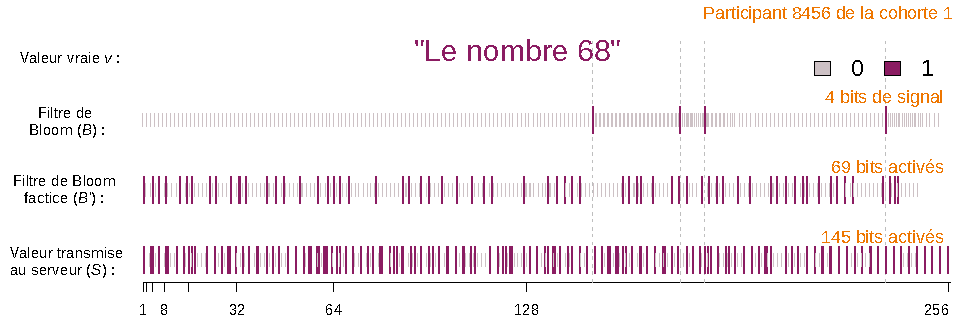
\includegraphics[scale=0.78]{schema_RAPPOR.pdf}
\end{center}
%
\subsection{Versions modifiées}
%
Cet algorithme reste adaptable selon le scénario:
\begin{itemize}
    \item 
    \textbf{Collecte unique}: par nature, la protection longitudinale est inutile. On peut sauter l'étape 2 (donc choisir $f=0$).
    \item 
    \textbf{Collecte basique}: il s'agit du cas où l'ensemble de chaînes relevées est assez petit et où chacune peut être représentée par un bit unique dans un tableau (le genre d'une personne par exemple). 
    Dans ce cas, l'utilisation du filtre de Bloom est inutile. 
    On la remplacera par la traduction déterministe de chacune des valeurs en un unique bit de $B$ (d'où $h=1$).
    \item 
    \textbf{Collecte basique unique}: combinaison des précédentes, c'est le cas le plus simple envisageable.
\end{itemize}
%
\subsection{Influence des paramètres}
%
\subsubsection{Epsilon}
%
Notons que le choix de $\epsilon$ n'est pas trivial, faute d'être immédiatement interprétable: l'article de Justin Hsu \textit{et al.}~\cite{HGHK14} en $2\,015$ semble être le premier consacré à cet objectif et fait état de la complexité de la détermination de ce réel, en l'absence d'une sémantique évidente.
Cet unique curseur doit en effet correspondre à des situations et des intérêts divers: l'analyste attend un maximum de précision de ses statistiques, tout en puisant le moins possible dans son \og budget de confidentialité\fg{}. 
L'utilisateur qui cède ses données, même avec une contre-partie, désire la plus grande confidentialité possible. 
Et la prise de risque acceptable sera fonction de la nature des données à protéger. 

Hsu constate (\cite{HGHK14} tableau 1 page 24) que  dans la littérature $\epsilon$ peut facilement varier de $0,01$ à $10$, sans qu'une justification ne soit toujours apportée! Dans l'article d'Erlingsson qui présente RAPPOR~\cite{EPK14}, c'est $\epsilon=\ln 3$ qui est choisi pour les expérimentations.
%
\subsubsection{Utilisation de cohortes}
%
Le but d'une étude conduite avec RAPPOR est généralement de déterminer quelles chaînes sont présentes et à quelle fréquence, dans la population étudiée. 
On cherche donc à réduire le taux de faux positifs (dus au filtre de Bloom). 
À cet effet, on partitionne aléatoirement la population sondée en $m$ cohortes d'effectifs similaires.
Chacune utilise un ensemble de fonctions de hachage qui lui est propre pour son filtre, afin de réduire les collisions de chaînes d'une cohorte à l'autre. 

Les faux positifs augmentent quand $m$ est trop petit, mais s'il est trop grand, chaque cohorte procure un signal insignifiant vu son faible effectif. Le choix de $m$ est donc important.
%
\subsubsection{Paramètres probabilistes et de configuration du filtre de Bloom}
%
Les paramètres $f$, $p$ et $q$ seront établis selon la valeur de $\epsilon$ désirée. On prendra en compte le fait que le taux de faux positifs (FDR, \emph{False Discovery Rate}) augmente proportionnellement à $f$. En l'absence de données longitudinales, on a vu qu'on peut opter pour la version \og collecte unique\fg{} de RAPPOR ($f=0$).

La taille $k$ du filtre de Bloom, la quantité $h$ de ses fonctions de hachages et le nombre $m$ de cohortes doivent également être fixées \textit{a priori}. Puisque ni $k$ ni $m$ n'interviennent au niveau de la détermination du cas le plus défavorable en termes de confidentialité, il seront choisis pour déterminer l'efficacité de la reconstruction du signal à partir de la sortie bruitée $S$. 
L'expérience indique que $h$ semble être le seul réellement déterminant en la matière (la plus petite valeur testée, $2$, semblant la meilleure au niveau utilisabilité compte tenu des autres paramètres choisis pour le test par Erlingsson\cite{EPK14}).


Au final, aucune règle évidente et automatique ne s'impose. La pratique restera prépondérante pour affiner ces paramètres.
%
\subsection{Confidentialité différentielle de RAPPOR}
%
Revenons sur la solidité de RAPPOR face aux diverses menaces envisageables.
%
\subsubsection{Garanties sur la réponse randomisée permanente}
%
Intuitivement, les étapes 1. et 2. contrent efficacement les adversaires exploitant les données longitudinales. Car comme on l'a mentionné, une analyse statistique permettrait au mieux de faire fi de l'étape 3 et de remonter à $B'$, mais pas à $v$, ni même à $B$.

Plus précisément, on montre que ces deux manipulations satisfont l'$\epsilon$-indiscernabilité, pour $\epsilon = 2h\ln\left(\frac{1-\frac{1}{2}f}{\frac{1}{2}f}\right)$, valeur qu'on notera $\epsilon_\infty$. Elle ne dépend que de $h$ et $f$. Une valeur faible de $k$ renforce la sécurité en augmentant les collisions dans le filtre de Bloom ---~et risque donc de nuire à l'utilisabilité de $S$~--- mais ça n'est ni nécessaire ni suffisant pour garantir l'$\epsilon$-indiscernabilité). 

Nous ne détaillons pas ici la preuve; elle repose sur les probabilités conditionnelles et l'indépendance d'événements, les calculs déjà évoqués autour de la réponse randomisée, et le fait que pour des positifs, on a $\frac{a+b}{c+d}\leqslant\max\left(\frac{a}{c},\frac{b}{d}\right)$ (\cite{EPK14} 3.1 page~5).

%
\subsubsection{Garanties sur la réponse randomisée instantanée}
%
Là encore, les deux étapes de randomisation forment une solide protection. 

On remarque que la probabilité $\mathbb{P}(S_i=1|B_i=1)$ qu'un bit soit à $1$ sur la sortie $S$ sachant qu'il l'est sur $B$ vaut $q^*=\frac{1}{2}f(p+q) + (1-f)q$ et que $\mathbb{P}(S_i=1|B_i=1)$ vaut $p^*=\frac{1}{2}f(p+q) + (1-f)p$.
Avec ces notations, il est alors prouvé que la réponse randomisée instantanée (étape 3) fournit la garantie de l'$\epsilon_1$-indiscernabilité, pour $\epsilon_1 = h\ln\left(\frac{q^*(1-p^*)}{p^*(1-q^*)}\right)$. La démonstration est analogue à une partie de la précédente.

En cas de réponses multiples, déterminer $\epsilon_n$ doit s'effectuer en prenant en compte la connaissance déjà apportée à l'adversaire. Déterminer des stratégies pour majorer cette valeur reste un chantier ouvert, en tout cas en $2\,014$.\\[-0.4em]

Comme on pouvait s'y attendre au vu de l'algorithme, les garanties offertes sont solides. 
De plus, cela a pu être rigoureusement justifié. 
Reste à vérifier qu'il est possible de tirer suffisamment d'informations pertinentes de données qui ont subi un tel traitement et à indiquer comment s'y prendre.
%% ========================================================================================== %%
%%
\section{Méthode RAPPOR -- L'exploitation des résultats}
%%
On rappelle qu'en général, le but est de savoir quelles chaînes sont présentes et à quelle fréquence, dans la population analysée. Vu les différentes étapes de transformation, l'utilisation d'outils statistiques avancés s'avère nécessaire.
%
\subsection{Étapes clés du décodage}
%
\begin{itemize}
    \item 
    En notant, pour une cohorte $j$, $t_{ij}$ le nombre de bits d'indice $i$ activés dans $B$ et $c_{ij}$ celui des bits $i$ à $1$ dans un ensemble de $N_j$ réponses, on peut estimer le premier par 
    \[t_{ij} = \frac{c_{ij} - (p+\frac{1}{2}fq-\frac{1}{2}fp)N_j}{(1-f)(q-p)}\]
    On note $Y$ un vecteur de $t_{ij}$, pour $i\in\llbracket1;k\rrbracket$ et $j\in \llbracket1;m\rrbracket$.
    \item 
    On crée une matrice $X$ de taille $km\times M$, où $M$ désigne le nombre de chaînes candidates. Elle est peu dense, avec beaucoup de $0$ et des $1$ associés au hachage du filtre de Bloom de chacune des chaînes de chaque cohorte.\\
    Une régression LASSO\footnote{\emph{Least Absolute Shrinkage and Selection Operator} est une méthode de régression qui fonctionne bien en grande dimension et permet de sélectionner au plus près possible un sous-ensemble restreint de variables par minimisation des carrés des résidus, ou tout autre méthode statistique analogue: \url{https://en.wikipedia.org/wiki/Lasso\_(statistics)}} permet d'ajuster un modèle $Y \sim X$ et de sélectionner ainsi les chaînes candidates associées aux coefficients non nuls. 
    \item 
    L'estimation des décomptes, ainsi que l'erreur standard et la $p$-\emph{value}, sont obtenues par la méthode des moindres carrés sur les variables sélectionnées.
    \item 
    Par correction de Bonferroni\footnote{Le but ce cette correction est d'éliminer des valeurs qui apparaissent comme potentiellement significatives, alors que cela n'est dû qu'à la multiplicité des tests sur les données traitées (un seuil de $0,05$ n'est alors plus adapté).\\Voir par exemple \url{https://www.stat.berkeley.edu/\~mgoldman/Section0402.pdf}} au seuil de $0,05/M$ \emph{(pour un choix classique de seuil} $\alpha=0,05$), on ne garde que les valeurs significativement non nulles d'un point de vue statistique.\\
    On peut également contrôler le taux de faux-positifs parmi les résultats \textit{a priori} significatifs (FDR) avec la procédure de Benjamini-Hochberg\footnote{\www{https://en.wikipedia.org/wiki/False\_discovery\_rate\#Benjamini\%E2\%80\%93Hochberg_procedure}{https://en.wikipedia.org/wiki/False\_discovery\_rate\#Benjamini-Hochberg\_procedure} ou \url{http://www.biostathandbook.com/multiplecomparisons.html}}
\end{itemize} 
%
\subsection{Évaluations expérimentales}
%
La pertinence de RAPPOR a été montrée~\cite{EPK14} sur les cas suivants. Pour chacun, on a choisi $p=0,5$ et $q=0,75$ (pour obtenir $\epsilon=\ln 3$):
%En version \og collecte basique unique\fg{} ($f=0$), on peut détecter environ $\sqrt{N}/10$ chaînes au maximum (atteint si la répartition est uniforme) sur un échantillon de taille $N$. Pour la version standard, c'est nettement moins.
\begin{itemize}
    \item 
    \textbf{Retrouver une distribution normale}: on a simulé une telle répartition aléatoire (avec $\mu=50$ et $\sigma=10$) sur $10\,000$ valeurs. Avec $f=0$, on constate que $10\,000$ données rapportées sont insuffisantes. $100\,000$ réponses font clairement apparaître la courbe en cloche sur une représentation graphique et un million en donent un tracé précis.
    \item 
    \textbf{Avec une distribution exponentielle}: un million de rapports sont collectées, sur autant de chaînes aléatoirement échantillonnées suivant une distribution exponentielle. On opte pour $f=0,5$, $h=2$, $k=128$ et $m=16$ cohortes. Après analyse avec la correction de Bonferroni, $47$ chaînes sont estimées comme significativement présentes, dont $2$ seulement sont des faux positifs. Les plus fréquentes sont particulièrement bien détectées ($p$-value $<10^{-10}$ pour le top $20$, $p$-value $<10^{-31}$ pour le top $10$) et toutes les chaînes présentes avec une fréquence supérieure à $1\%$ sont détectées. Celles de la \og queue\fg{} de la fonction de densité sont ignorées, protégées par le mécanisme de confidentialité.
    \item 
    \textbf{Cas réel: noms des processus sous Windows}. Il s'agit de $186\,792$ relevés sur $10\,133$ machines, listant les processus les plus actifs, pour identifier les plus populaires et estimer la fréquence d'un exécutif malicieux particulier. Avec $h=2$, $k=128$, $m=8$, $f=0,5$ pour $\epsilon_1\approx1,07$, $10$ processus ont été identifiés (fréquences de $2,5\%$ à $4,5\%$). La fréquence du \emph{malware} a pu être estimée à $2,6\%$.
    \item 
    \textbf{Second cas réel: pages d'accueil sous Chrome}. RAPPOR a été implémenté dans le navigateur, pour collecter quotidiennement auprès d'utilisateurs l'ayant accepté des réglages particuliers (qui peuvent être modifiés à l'insu de l'utilisateur par des logiciels malveillants, d'où l'intérêt d'un suivi), dont le choix de la page d'accueil. 
    Avec $k=128$, $h=2$, $m=32$ cohortes, $f=0,75$ pour $\epsilon_1\approx0,53$, sur une douzaine de millions de relevés, on obtient les résultats suivants: une page doit être signalée par environ $14\,000$ utilisateurs au moins pour être identifiée par RAPPOR; $31$ pages inattendues ont été relevées, certaines sur des domaines potentiellement malicieux. 
    Seules $0,5\%$ des URL candidates ont une présence suffisamment significative statistiquement, mais une fois réunies, elles représentent $85\%$ des fréquences relevées.
\end{itemize}

On constate que RAPPOR est adapté à diverses études de tendance, de distribution, ou de mise en évidence de faits anormaux, à condition qu'ils soient suffisamment fréquents. En effet, par nature, les données peu probables seront noyées dans le bruit assurant la confidentialité différentielle. 
%
\subsection{Limites de RAPPOR}
%
L'intérêt évident de cet outil et sa puissance prouvée n'en font pas une panacée. Il devra donc s'intégrer dans un ensemble de mesures diverses (celles déjà évoquées, ainsi que la décentralisation du stockage, sa limitation dans le temps, etc.)

En effet, certaines faiblesses subsistent. Par exemple, un utilisateur utilise parfois plusieurs terminaux. 
Cela permet en théorie de contourner la garantie de confidentialité par des requêtes sur différents canaux pour un même individu, même si en pratique il reste difficile de déterminer ces entrées associées.
Un choix de cohortes trop nombreuses et donc petites facilite le repérage d'une personne.
Une collecte de valeurs constantes partagées par tous les sondés avec un filtre de Bloom trop grand permet un suivi individuel car les bits de la réponse randomisée permanente sont alors corrélés.
Tous ces points pourrait affaiblir la confidentialité, dans l'absolu. Plusieurs peuvent cependant être évités ou atténués par des mesures additionnelles.

Un point fort de RAPPOR est de pouvoir fonctionner côté client, en laissant potentiellement l'utilisateur d'un LBS paramétrer lui-même le risque admis. 
Mais cela reste très théorique car la sémantique de $\epsilon$ est hors de portée de la plupart des individus. 
Sans compter qu'au delà des conséquences directes d'une perte de confidentialité, on ne réalise généralement pas tout ce qui peut en être déduit. 
L'utilisateur insuffisamment éclairé risque donc d'être contraint de s'en remettre au LBS et de lui faire confiance, alors que leurs intérêts ne convergent pas nécessairement.

En ce qui concerne l'installation proprement dite, un dépôt {GitHub} est idéal. Mais celui de RAPPOR commence à dater: il n'a pas fonctionné tel quel en ce qui nous concerne et il a fallu modifier certains scripts et revenir à des versions plus anciennes de {Python} par exemple. C'est un peu secondaire, mais une mise à jour du processus d'installation serait intéressante.

Un dernier point semble particulièrement important au regard de notre projet: la protection concernant les données longitudinales n'est effective que si l'on se base sur la réponse randomisée permanente.
En cas de variation rapide de la valeur véritable pour un individu donné, cette garantie n'est plus applicable sans prendre des mesures particulières. 
Ne dépenser qu'une petite partie du budget $\epsilon_\infty$ à chaque rapport, au fil du temps, se traduirait par des valeurs de $q$ de plus en plus proches de $p$. 
Nous devrons certainement approfondir cette réflexion pour pouvoir travailler avec des données longitudinales de localisation. 
La réflexion portera également sur la représentation de ces valeurs, ainsi que les utilisations qui peuvent en être faites et donc les caractéristiques à conserver au mieux.\\[-0.4em]

La tâche s'annonce ardue mais passionnante!
\newpage
\bibliographystyle{plain}%  unsrt pour l'ordre des citations sinon plain
\bibliography{jmg}
\end{document}
